% This file was created by matlab2tikz.
%
%The latest updates can be retrieved from
%  http://www.mathworks.com/matlabcentral/fileexchange/22022-matlab2tikz-matlab2tikz
%where you can also make suggestions and rate matlab2tikz.
%
\documentclass[tikz]{standalone}
\usepackage[T1]{fontenc}
\usepackage[utf8]{inputenc}
\usepackage{pgfplots}
\usepackage{grffile}
\pgfplotsset{compat=newest}
\usetikzlibrary{plotmarks}
\usetikzlibrary{arrows.meta}
\usepgfplotslibrary{patchplots}
\usepackage{amsmath}

\begin{document}
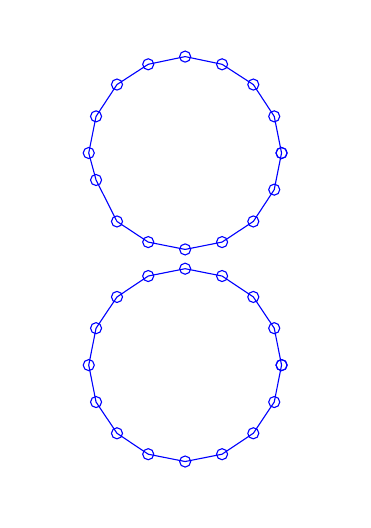
\begin{tikzpicture}

\begin{axis}[%
width=4cm,
height=6cm,
at={(0cm,0cm)},
scale only axis,
axis equal,
xmin=-1.1,
xmax=1.1,
ymin=-1.4,
ymax=3.5,
axis line style={draw=none},
ticks=none
]
\addplot [color=blue, mark=o, mark options={solid, blue}, forget plot]
  table[row sep=crcr]{%
1	0\\
0.924	0.383\\
0.707	0.707\\
0.383	0.924\\
6.12e-17	1\\
-0.383	0.924\\
-0.707	0.707\\
-0.924	0.383\\
-1	1.22e-16\\
-0.924	-0.383\\
-0.707	-0.707\\
-0.383	-0.924\\
-1.84e-16	-1\\
0.383	-0.924\\
0.707	-0.707\\
0.924	-0.383\\
1	-2.45e-16\\
};
\addplot [color=blue, mark=o, mark options={solid, blue}, forget plot]
  table[row sep=crcr]{%
1	2.2\\
0.924	2.58\\
0.707	2.91\\
0.383	3.12\\
6.12e-17	3.2\\
-0.383	3.12\\
-0.707	2.91\\
-0.924	2.58\\
-1	2.2\\
-0.924	1.92\\
-0.707	1.49\\
-0.383	1.276\\
-1.84e-16	1.2\\
0.383	1.276\\
0.707	1.49\\
0.924	1.82\\
1	2.2\\
};
\end{axis}
\end{tikzpicture}%
\end{document}